\documentclass[11pt, a4paper]{article}
\usepackage[utf8]{inputenc}
\usepackage{graphicx}
\usepackage{amsmath}
\usepackage{float}

\title{EE20B051 ASSIGNMENT 3}
\author{Jineeth N (EE20B051)}
\date{ 18th February 2022}

\begin{document}

\maketitle

\section{AIM:}
    The aim of the assignment is:
    \begin{itemize}
        \item To analyse the give noisy data and plot the graphs of the data.
        \item  To Observe the error in fitting the Least Error Fit function for the given set of data.
        \item To Find the relation between the error observed and the noise in the data.
        \item Get used with matplotlib library
    \end{itemize}
     
\section{Observation:}
       The function which is used is:
        \begin{equation}
            f(t) = 1.05J_2(t)-0.105t
        \end{equation}
        where $J_2(t)$ is the \textit{Bessel Function of the first kind of 2nd order}. we can obtain the true data using this equation.
        
        
     
        \subsection{Importing and plotting the given data:}
            \item First the data in \textbf{fitting data}   file is being uploaded into the program. This has data that is being stored in columns out of which the first columns contains the time values and the other columns contain the noisy data.The plot of the noisy data and the true value against the time axis is shown in the below diagram:
        
        \begin{figure}[H]
            \centering
            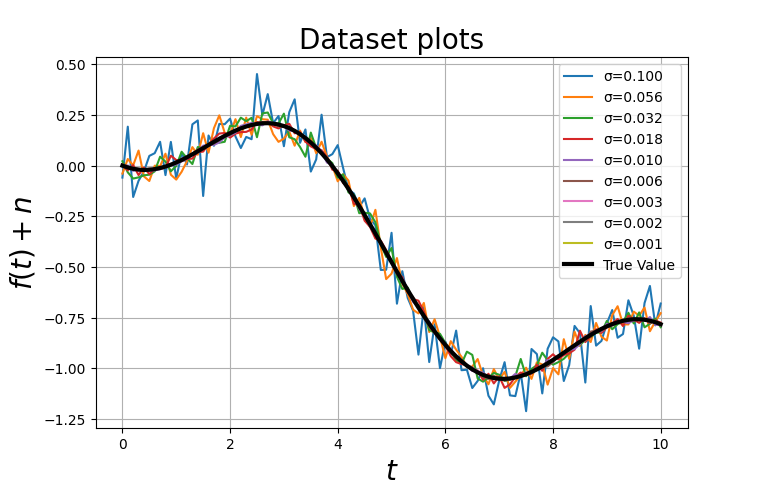
\includegraphics[scale=0.75]{Figure_0.png}
            \caption{Noisy Data with True Data}
            \label{fig:noisyAndTrue}
        \end{figure}
        
        
        By the above above graph we can say that as the value of σ increases the data becomes more noisier.The below plot is the \textit{Errorbar plot} of the first coloumn of noisy data with the true value against the time axis.
        
        \begin{figure}[H]
                \centering
                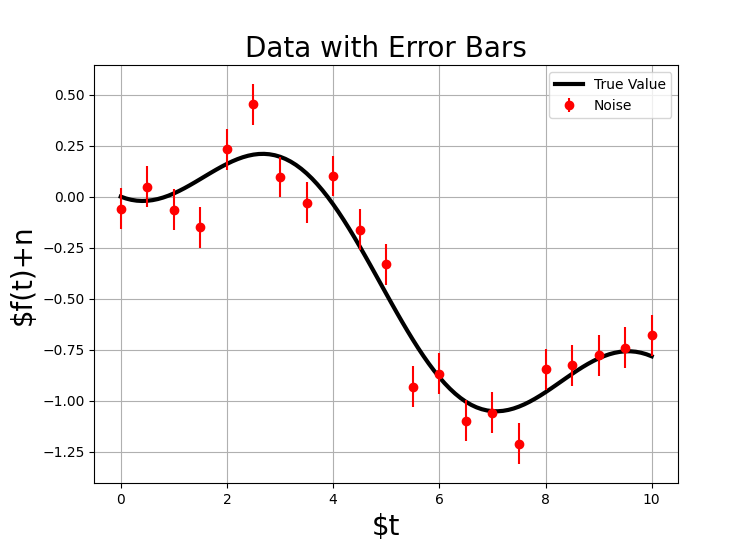
\includegraphics[scale=0.75]{Figure_1.png}
                \caption{Noisy Data with Errorbar}
                \label{fig:noiseError}
            \end{figure}
            
        The red lines (\textit{error bar}) in the above plot indicate the standard deviation of the noisy data from the original data, at that value of $t$.To make the plot more readable it is plotted at every $5^{th}$ point.
        
        \subsection{Calculating RMS error for different values of A and B:}
        
        From analyzing the data, we can understand that the noisy data can be approximately fitted into a function shown below:
        \begin{equation}
                g(t, A, B) = AJ_2(t)+Bt
            \end{equation}
            where A and B are constants, which are to be found using graphical and least
square fit function of the python.
            To find the coefficients A and B,we will find the mean square error between
the noisy data (1st column) and the function for a range of values of A [0,0.1,0.2
... 2] and B [-0.2,-0.19,-0.18,....,-0.01,0], which is given by:

            \begin{equation}
                \epsilon_{ij} = \frac{1}{101}\sum_{k=0}^{101}(f(t_k) - g(t_k, A_i, B_j))^2
            \end{equation}
        where $\epsilon_{ij}$ is the error for $(A_i,B_j)$.
        
        The contour plot of the error is shown below

        \begin{figure}[H]
                \centering
                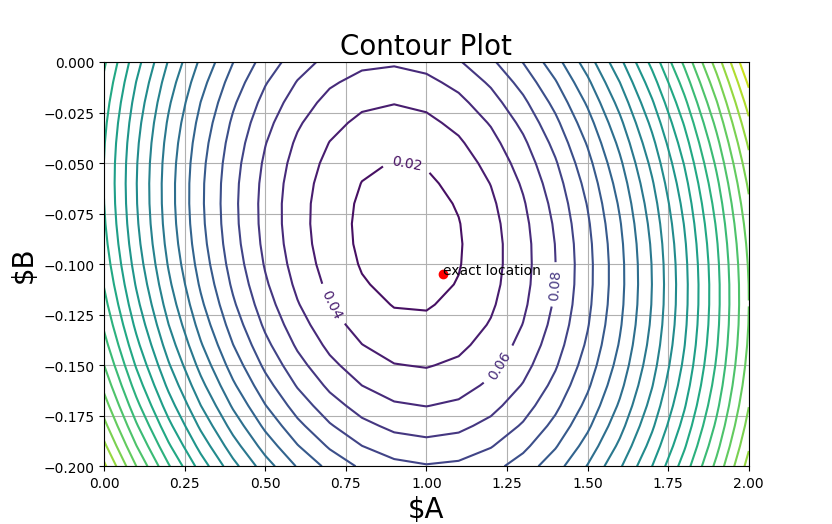
\includegraphics[scale=0.75]{Figure_2.png} 
                \caption{Contour Plot of $\epsilon_{ij}$}
                \label{fig:contourPlot}
            \end{figure}
            
            
            
            
            We can observe that the location of the minima is approximately near the orignal function coefficients.
            
        \subsection{Finding out the variation of $\epsilon$ in estimation of A and B w.r.t $\sigma_n$: } 
        
        We find that the variation of the mean squared error of values $A_p$ and $B_p$ is as follows:
        
            
        \begin{figure}[H]
                \centering
                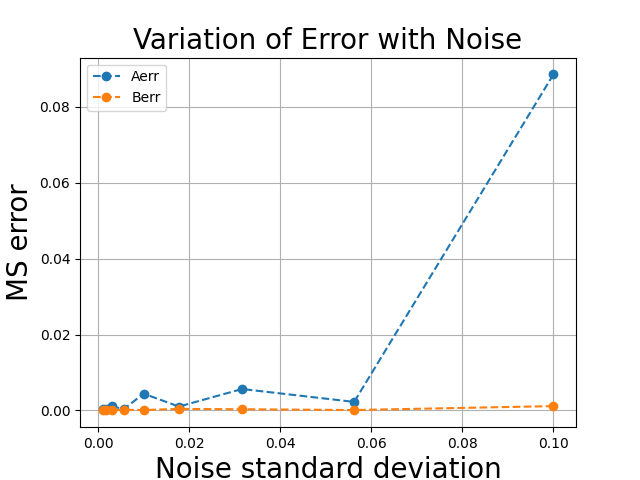
\includegraphics[scale=0.75]{Figure_3.png} 
                \caption{Mean Squared Error vs Standard Deviation}
                \label{fig:errorSTD}
            \end{figure}
            
        By observing the above graph we can conclude that the plot doesn't give essential relationship between $\sigma_n$ and $\epsilon$. To get the more accurate plot we can use loglog plot which will give the below output
        
        \begin{figure}[H]
                \centering
                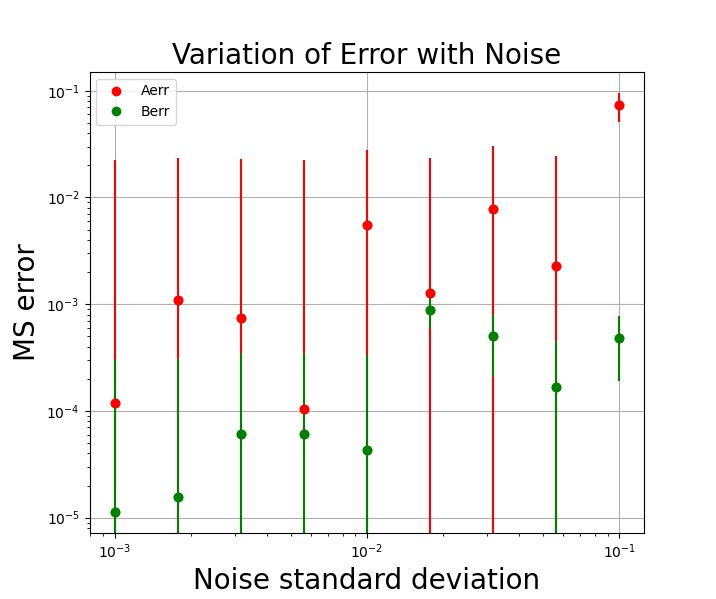
\includegraphics[scale=0.5]{Figure_4_1.jpeg} 
                \caption{Error vs Standard Deviation \texttt{loglog} Plot}
                \label{fig:errorSTDloglog}
            \end{figure}
            
        From the above plot we can observe that we are approximately getting linear relationship between $\sigma_n$ and $\epsilon$.
        
    \section{Conclusion}
        The given noisy data was extracted and the best possible estimate for the
underlying model parameters were found by minimizing the mean squared
error. This is one of the most general engineering use of a computer, mod-
elling of real data.we also found that error in estimation of A and B is increasing with standard deviation and it is non linear.
\end{document}
